\documentclass[a4paper]{article}

%% Language and font encodings
\usepackage[english]{babel}
\usepackage[utf8x]{inputenc}
\usepackage[T1]{fontenc}


%% Sets page size and margins
\usepackage[a4paper,top=3cm,bottom=2cm,left=3cm,right=3cm,marginparwidth=1.75cm]{geometry}

%% Useful packages
\usepackage{natbib}
\usepackage{graphicx} 
\usepackage{listings}
\usepackage{color}
\usepackage{amsmath}
\usepackage{float}
\usepackage{commath}
\usepackage{upgreek}
\usepackage[numbib]{tocbibind}
\usepackage{hyperref}
\usepackage[font=sc]{caption}
\usepackage[justification=centering]{caption}

\title{Deep Neural Networks: A Visualization and Comparison with Shallow Neural Networks\\ \large Tutored Research Project II}
\author{Candice Bent\'ejac, Anna Cs\"org\H o, D\'aniel Hajt\'o \\Tutored by Vincent Lepetit}

\begin{document}
\maketitle

\begin{abstract}
This report presents our work our Tutored Research Project on Deep Neural Networks. We try to get a better understanding of how neural networks are mapping and tuning their parameters through the visualization of their decision boundaries, layer by layer. For this purpose, we develop a Python library that allows such a visualization. We also try to determine, through experiments, if deep networks are, as the recent works lead us to think, indeed better at problem solving than shallow ones by approximating grayscale images. 
\end{abstract}

\section{Introduction}
%%% Upside-down pyramid which contains a description of our domain (deep neural networks), presents our topic (visualization of networks and intuition that deeper networks generalize better than large and shallow ones. Present our outline in a fancy and exciting way.

% Description of the domain
\paragraph{}Neural Networks, or more properly, Artificial Neural Networks (ANN), are computational models that are loosely based on the neural networks that can be found in mammals' brains. Not only do those natural neural networks allow us to process information, but they also make us able to learn, an ability computers are lacking of. Indeed, unlike the brain as a biological neural network that can reorganize itself and learn to compensate errors, computers are dependent on us to formulate problems as algorithms before being able to solve them. However, we are not able to  formulate any problem as an algorithm, especially problems depending on many variables. This causes computers to fail solving some problems where a human brain would succeed. \citep{Krose1996}

\paragraph{}ANN are thus trying to mimic, on a smaller scale, the behavior of the mammalian brain when facing a problem. They are aiming at allowing, abstractly speaking, a computer to learn by itself, as our brain would. They do not need to be explicitly programmed: they are able to learn from training examples. More precisely, they are able, after a successful training, to generalize a problem and associate data by themselves, without further human intervention. This allows ANN to solve problems where other computational models are struggling or failing.

\paragraph{}ANN are typically constituted of layers, which themselves consist in interconnected nodes, often designated as "neurons". The input to an ANN is presented to the input layer, which then communicate with one or more hidden layers. The real processing of the input happens within those hidden layers, where all the computations are done. The hidden layers finally communicate the result of their computation to the output layer, which will return it. \citep{Kriesel}

\paragraph{}There are different types of ANN, but the ones that generated the most excitement recently are Deep Neural Networks (DNN), which are ANN with many hidden layers. DNN even led to the creation of a new branch of machine learning: deep learning. Thanks to deep learning, many breakthroughs have been made in domains such as computer vision or speech recognition, which explains the keen interest people have developed for it.

\paragraph{}If DNN, and more generally ANN, have proven themselves to be an efficient model to solve problems, they are yet still behaving as black boxes. We are able to understand the mathematics behind ANN, but fail to predict how the networks map and tune their parameters because of the infinite number of possibilities. 

% Presentation of our topic
\paragraph{}In this report of our Tutored Research Project, we focus on two specific concerns that the study of ANN is raising. The first one is about the networks' visualization: in order to better understand how the ANN are optimizing themselves, we might want to gain insights from a direct visualization of the decisions that the networks are taking. To that effect, we will build a library that allows its users to precisely visualize the decision boundaries that a given network is determining for each of its layers. The second of our concerns regards the type of network that has the best ability to approximate functions. We thus will make a comparison between two different types of network's structures: a shallow one (regular ANN) and a deep one (DNN). Putting them through the same training and testing conditions, we will attempt to approximate grayscale images of different difficulties (synthetic images, synthetic textures and real images) and try to draw a general conclusion based on our results about which network's structure seems to be more adapted to problem solving.

% Outline
\paragraph{}To start with, we will therefore review the already existing visualization solutions as well as the studies that have been conducted on the correlation between a network's structure and its ability to generalize. The following section will be dedicated to describing the requirements we had to follow for both of our tasks, before describing the software architecture of Pear, our library. We will then comment our implementation and finally, present the tests we ran and the results we obtained.




\section{State-of-the-art and existing solutions}
% Can be a synthesis of the work done in Madrid but irrelevant in our case. 
%- for the visualization part, there are not really existing solutions to the precise things we want to achieve, but the TensorFlow Playground is already a good and interesting neural network visualization tool that might be worth mentioning.

\paragraph{}The questions of visualization and ANN's structure we stated earlier have already been studied. We however noticed that those specific points had not been widely covered: we could not find any work addressing the problem of visualization the way we do, and the comparisons of deep and shallow networks we read about were mostly written by the same researchers. In this context, our own work becomes relevant, since its intent is to hopefully complete what has already been uncovered rather than presenting it in another way.

\paragraph{}Throughout this section, we will thus present the already existing solutions to the visualization and structure problems, starting with the visualization methods for Deep Neural Networks before speaking of the different comparisons that have been already made between deep and shallow networks.  


\subsection{Visualization of Deep Neural Networks}
\paragraph{}Visualization methods for DNN, and more generally ANN, are relevant, since they might help us getting a better understanding of how the networks are operating and adapting, and what makes them such powerful models. Obtaining this knowledge is important for various reasons. One of the most important is that, so far, trial-and-error is the main way to find the best set of parameters when training an ANN. Besides being time-consuming, it results in networks having thousands or millions of parameters, which only makes it harder to improve them. Indeed, the higher the number of parameters, the harder it gets to find the strengths and weaknesses of the networks. Understanding how the networks are actually learning is thus necessary to improve their training phase and, by extension, improve networks which have already, through trial-and-error, proven themselves to be successful.

\paragraph{}In this context, \citep{ZintgrafICLR2017} and \citep{Zintgraf2017} present a recent method to visualize the response of a DNN to a specific input. For example, when inputting an image, the method will highlight the areas of the image that provide information in favor of or against a certain class. This type of visualization leads to a better understanding of the classification process which the neural network goes through, and how and why a class is chosen rather than another. 

\paragraph{}Another approach to visualize Deep Neural Networks is to focus on the notion of a class, that is to say, what a network understands to be a class. For a given class, it consists in finding an input that will maximize this given class. We can then visualize what the network is looking for in an image to then classify it, and thus have an idea of what specifically triggers the network when attempting to classify. \citep{Simonyan2014} use this approach to develop two visualization techniques for Convolutional Neural Networks (CNN). The first one visualizes the notion of the class that a CNN has by generating an image that maximizes the class score for a given class. The second one is an image-specific class saliency visualization that computes the given class saliency map by ranking the input features, depending on their influence over the given class. \citep{Yosinski2015} also introduce two visualization techniques. One visualizes the activations that are made by a CNN as it processes an image or a video, which allows to gain valuable insights on those networks work. The other consists in visualizing the features at each layer of a DNN. To this end, it performs regularized optimization in the image space.

\paragraph{}It seems also important to note that there are very few accessible visualization tools available on-line for a large public that does not necessarily have a great knowledge about Deep Neural Networks. One tool worth mentioning for people willing to familiarize themselves with ANN and others willing to play around with them is the TensorFlow Playground \citep{TFPlayground}. It allows the user to choose between simple datasets, select how many hidden layers and neurons they want to use, and to set several parameters, including the activation function and the learning rate. Once all the parameters have been set, the Playground displays the network's output for each epoch and lets the user visualize the output of each neuron on each layer.

\subsection{Comparison between deep and shallow networks}
\paragraph{}The depth of DNN has greatly evolved over the past few years. The now well-known AlexNet \citep{Krizhevsky2017} won the 2012 ILSVRC (ImageNet Large-Scale Visual Recognition Challenge) with 7 hidden layers, outperforming by more than 10 percent the other contestants. In 2015, Microsoft ResNet \citep{He2016} won the ILSVRC using 152 layers. Between 2012 and 2015, the winners of each ILSVRC (ZF Net \citep{Zeiler2014} (winner in 2013), VGG Net \citep{Simonyan2015} (runner-up in 2014) and GoogLeNet \citep{Szegedy2015} (winner in 2014)) used networks with an increasing number of layers, always achieving better results than those from the previous years. This suggests that deep networks are, at least in the context of image recognition, better than shallow ones and that, the more layers a network has, the better it will perform. 

\paragraph{}\citep{Zagoruyko2016} however shows that a deep residual network with "only" 16 layers can outperform all the previous residual networks, even those having a thousand of layers, both in accuracy and efficiency. This indicates that although a deep network seems to perform better than a shallow one, the performance is not determined by the number of layers itself.

\paragraph{}Furthermore, \citep{Mhaskar2016} and \citep{Mhaskar2016May} show that a shallow network and a deep network can approximate the class of compositional functions with the same accuracy. However, a deep network will achieve such a result with an exponentially lower number of training parameters and a lower VC-dimension (given a space of functions that can be learned by a statistical classification algorithm, the VC-space measures that space and consists in the cardinality of the largest set of points that the algorithm can shatter). % reformulate the definition of VC-space: might be too close to the wikipedia one 
\citep{Poggio2017} and \citep{Mhaskar17} further discuss when and under which conditions learning with deep networks can be exponentially better than learning with shallow ones. 

\paragraph{}They state that both shallow and deep networks are universal and can thus approximate arbitrarily well any continuous functions on a compact domain (universal approximation theorem) and consider a class of functions on a compact domain that is a hierarchical composition of local functions. When approximating those functions with a compositional structure, deep networks can represent compositionality in their architecture whereas shallow networks cannot do so and thus do not have any structural information on the function to be learned. Moreover, deep networks are able to exploit the special structure of compositional functions in their architecture when shallow networks are plainly blind to it. It is also not a requirement for the deep networks to have the same compositional architecture as the compositional functions to be approximated: the acyclic graph representing the structure of the function only needs to be a subgraph of the graph representing the deep networks' structure.

\section{Software requirements}
\paragraph{}Our research project is divided into two main parts. The first one consists in building a library that could be used by anyone willing to work with neural networks and to improve their network during their optimization phase. In order to do that, the library will allow the user to visualize the neural network's decision boundaries. Additionally, we will develop a program using that library that lets the user give a file containing a network's parameters as an input, and draws its decision boundaries as a means of visualization of its organization. The second part consists in checking experimentally whether small and deep networks tend to generalize better than large and shallow ones. For this, we will build different networks and evaluate their ability to approximate grayscale images of various difficulties. We will then build plots out of our test results to analyze them and assess our intuition.

\paragraph{}In this section, we will present our requirements, listing for each part of our project the constraints, the functional needs, and the non-functional needs. 

\subsection{Network visualization}
\subsubsection{Constraints}
\begin{itemize}
\item The library and the program will both be developed using Python.
\item The networks involved should only use the Rectified Linear Unit (ReLU) operator. 
\item The program should only take as an input a network and its parameters saved in a TensorFlow file.
\item The program should display all the layers of the network with different colors.
\end{itemize}

\subsubsection{Needs}
\noindent\textbf{Functional needs}
\begin{itemize}
\item The library should be able to be called by a user building their own networks and trying to optimize them by using visualization.
\item The program should have a graphical user interface (GUI).
\item The program should display the network, given as an input by the user, by drawing all its decision boundaries for all neurons, on all layers. 
\item The program should be able to display all the layers and neurons at the same time if requested by the user, no matter how big the input network is.
\item The user should be able to choose which layer are being displayed by the program. 
\item The user should be able to save the network visualization displayed by the program as a .jpg image.
\item The user should be able to choose which part of the plane shown by the program they want to see and change it as they want. By default, the region of the plane to be shown will be set automatically. 

\end{itemize}
\noindent\textbf{Non-functional needs}
\begin{itemize}
\item For each region displayed by the program, the slope of the visible decision boundaries should also be displayed.
\end{itemize}

\subsection{Part II}
\subsubsection{Constraints}
\begin{itemize}
\item The experiments should be developed and run using Python.
\item All the neural networks built for the experiments should be created and used with TensorFlow.
\item All the images used for our experiments should be of a format that can be handled by TensorFlow neural network. 
\item All plots should be plotted using Matplotlib.
\item Only grayscale images should be used as inputs for our experiments.
\item The images used as inputs for our experiments should be of different types and difficulties: synthetic simple images (such as a black square on a white background), synthetic images with noise, synthetic textures, and real images.
\item The method of least squares should be used to evaluate the networks' abilities to approximate the input images.
\item The smooth L1 norm should be used as the loss function to evaluate the networks' abilities to approximate the input images.
\item A single network should be used for a single image.
\end{itemize}

\subsubsection{Needs}
\noindent\textbf{Functional needs}
\begin{itemize}
\item Neural networks should be created, trained on images, and their ability of approximating those images should be assessed. 
\item A parameter should determine how many percents of the input image's pixels will be used for the training phase.
\item 100\% of the input image's pixels should be used during the testing phase.
\item The input of a neural network should be the location of an input image's pixel.
\item For one experiment with a given input, the same number of parameters should be used for all the networks. Only the structure of the networks should vary.
\item The generated plots should be the curves of the least square error (on the $y$ axis) depending on the number of layers and the total number of parameters (on the $x$ axis). A curve should correspond to a specific number of layers.
\item On every plot, each point in the curve should be an average over several trials using different training sets.

\end{itemize}

\section{Software architecture}
%(ULM schemes), how our software is organized, what our modules are. Also insert a magnificently beautiful Gantt chart.
\paragraph{}Our work spanned over several weeks. The way we distributed and organized it is shown in the Gantt chart of Figure XX. (Insert beautiful updated Gantt chart here -- see how to split it so that the X pages remain readable on a figure) Within this section, we will dive into the architecture of our project, and more specifically, of Pear, our ANN visualization library. The comparison we made between the deep and the shallow networks is based on experiments and analysis of their results only, which means that it does not have a dedicated software architecture. We will however briefly mention its organization.

\subsection{Pear: a visualization library}

\paragraph{}The library aimed at ANN visualization we wrote obeys to the rules of modular programming. It is consequently constituted of different modules which have specific goals. Figure \ref{fig:modules} shows the relations between these modules within Pear, and more generally, the interaction between Pear and other external libraries that are required to get ours to work.

\begin{figure}[h]
\centering
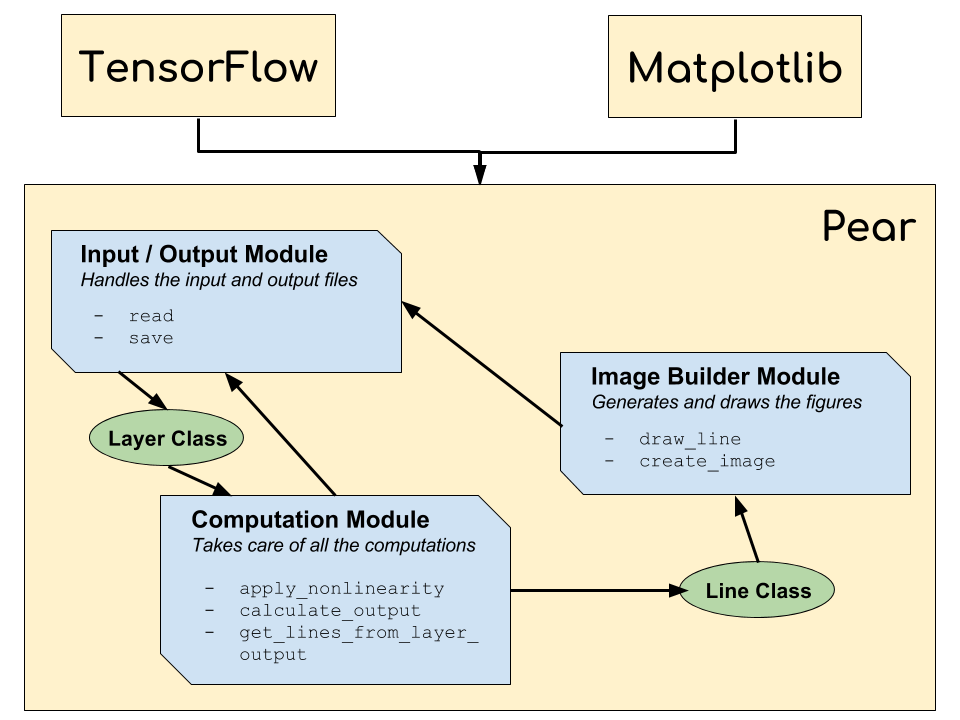
\includegraphics[scale=0.3]{images/Modules.png}
\label{fig:modules}
\caption{The images used to test the approximating capability of the different networks.}
\end{figure}

\subsubsection{Pear's modules}
\paragraph{}Pear relies on three main modules: the Input / Output module, the Computation module and the Image Builder module.
\begin{itemize}
\item The Input / Output module handles exclusively what the user gives as an input (TensorFlow files) and what the user receives as an output (the visualized input network, or the computations made on every layer to obtain the decision boundaries). It focuses on reading and parsing the input TensorFlow files before transmitting them to the Computation module. The Computation or the Image Builder module, depending on what use the user wants to make of the library, will then send the output back to it. The Input / Output module also makes use of our \verb?Layer? class, which we use to properly handle the weight and bias matrices of every network's layers.
\item The Computation module aims at applying the non-linearity operator (in our case, ReLU) to all neurons and then compute the output of the layers for all the possible inputs. With these outputs, it then is able to compute the lines that correspond to the network's decision boundaries. Depending on what the user wants, it can either give the output back to the Input / Output module, or send it to the Image Builder module to get a visualization of it. The Computation module uses our \verb?Line? class to have a structure associated with the decision boundaries. 
\item The Image Builder module is in charge of the drawing of the decision boundaries for each layer. Given the results computed by the computation module, it draws the decision lines accordingly for the requested layers. It then transmits the created image to the input/output image. The Image Builder module receives \verb?Line? instances created by the Computation module as an input, because in case the user would want to proceed to a visualization of the network, the use of the \verb?Line? class makes the figure generation easier by directly formatting the Computation module's output into data that is more adapted to plotting.
\end{itemize}
The executable uses all of these modules within a graphical user interface.

\subsubsection{Dependency on other libraries}
\paragraph{}Pear uses two external libraries: TensorFlow \citep{tensorflow2015-whitepaper} and Matplotlib \citep{Hunter:2007}. 

\paragraph{}TensorFlow is used by the Input / Output module to read in files containing ANN created in and with TensorFlow. Indeed, TensorFlow has its own file representation -- a graph representing the network's structure -- and saves networks as binary files which cannot be read without it. 

\paragraph{}Regarding Matplotlib, it is only used by the Image Builder module. Matplotlib being popular, well-documented and providing many functions that were relevant to our uses (figure creation, figure updating, easy navigation within a figure, etc.), we decided to directly use it to generate our plots rather than implementing it again on our own. 


\subsection{Comparison between deep and shallow networks}
\paragraph{}This part of our work being test-driven, we organized it according to our test images. We used three categories of images (synthetic images, synthetic textures and real-world images) and for each image, we used dedicated weights on a deep and on a shallow network. To be deepened and better formulated...


\section{Implementation}
%Explain which algorithms we used or what algorithms we wrote specifically for our project. Basically, speak of the code content in a comprehensive and appealing way.
\paragraph{}In this section, we go into the implementation details of both Pear (and its executable) and the tests used to compare deep networks with their shallow counterparts. We developed them using Python only, associated to Google's TensorFlow and Matplotlib libraries, and Tkinter \citep{Hughes:2000:PTP:350314.350415} for the graphical user interface.

\subsection{Pear: a visualization library}
\paragraph{} For Pear's implementation to be clearer, we will go through each module's implementation individually. 

\subsubsection{Classes}
\paragraph{\textit{Layer}} In order to handle the layers of the neural network compactly we defined a class for the layers.
Each \textit{Layer} object has a weight matrix (\textit{W}) and a bias vector (\textit{b}). We also store the number of inputs the layer takes ($n\_input$), which is equal to the number of columns in the weight matrix, and the number of neurons in the layer ($n\_neurons$). which is equal to the number of outputs the layer will produce (number of rows in the weight matrix). A color value is also associated for each layer. We will use this color value later to draw the boundary lines to the image with a unique color. To define a $Layer$ object, in the constructor, the weight matrix, the bias vector and the color value should be given. 
Each $Layer$ object is able to calculate its own output by its function $calculate\_layer\_output\_mat$. The function can handle several input points in the same time. The inputs should be given in an array, where each column corresponds to an input point. (The array should have $n\_input$ row.) The function returns an array, containing in each column the output of the layer for the given inputs in the same order. (The returned array will contain $n\_neurons$ row, and the same number of columns as the input did.) The output is calculated in the following way:

\begin{equation}
h = W x + b,
\label{eq:layer_output}
\end{equation}
where $h$ is the output of the layer, $W$ is the weight matrix, $x$ is the input, and $b$ is the bias vector

\paragraph{\textit{Line}}
The $Line$ class was created in order to make the handling the drawing of a line/broken line simply and uniformly. A $Line$ object contains the coordinates of the points which are belonging to the boundary on an image ($points$). %TODO extend this when its done. Add the sign attribute if necessary


\subsubsection{Input / Output module}
\paragraph{}This module contains the functions related to file handling, meaning the the reader function, which is responsible for reading a TensorFlow file, an the saver function, which can be used to save the generated image. The library resorts to TensorFlow in this module only. Indeed, the files that can be given as an input are TensorFlow files, which are binary files, and require the use of the external library to be read. Out of these binary files, we extract the parameters and returns them to the computation module, which will proceed to all the necessary calculations.


\paragraph{\textit{read\_file}}
The input of this function is the name of the TensorFlow file to read. %TODO Description how the function opens/reads the file...
Our representation of the network is a list of layers, containing the layers in order, meaning that the $i^{th}$ element of the list is the $i^ {th}$ layer.

\paragraph{\textit{save\_image}}
The function saves the given image on the specified filename given in its parameter in .png format. % TODO extend if it is ready


\subsubsection{Computation module}
\paragraph{}The Computation module consists in two main tasks: applying the non-linearity operator, which we chose to be the rectified linear unit (ReLU), and computing the decisions made by the network for every layer that is asked by the user.

%\paragraph{}Description of ReLU ($0$ if $h <= 0$, $h$ if $h > 0$) and of how the output of a layer is computed, given the weights and bias of it (and of the previous layers).

\paragraph{\textit{apply\_nonlinearity}}Applies the rectified linear unit (ReLU) function for its input given in its parameter. The ReLU function is defined by Equation \ref{eq:ReLU}:

\begin{equation}
\left\{
  \begin{array}{lr}
  	h & : h > 0\\
    0 & : h \leq 0,
  \end{array}
\right.
\label{eq:ReLU}
\end{equation}
where $h$ is the input.

\paragraph{\textit{calculate\_output}}This function calculates the output of a given layer for all the possible input pairs in the given range. The parameters of the function are the index of the layer for which we would like to calculate the output ($layer\_idx$), the ordered list of the layers at least until the queried layer index ($theta$) and the size of the region for what we would like to calculate the output, (size of the image) ($size$).

First, the function calculates all the possible input pairs in the range of $(0, size)$ % Maybe -if we will have it- talk about the resolution
and initialize the $h\_new$ matrix, which will contain an input pair in each column.

Then we will iterate over the layers until the queried one.
In each iteration, the $h\_new$ matrix will be updated with the output of the next layer, so we will store the output of the current layer in $h\_old$ by copying $h\_new$ to $h\_old$ at the beginning of the iteration.
Then we calculate the output of the next layer considering as input the output of the previous layer by calling its function $calculate\_layer\_output\_mat$ with $h\_old$. We save the new output values into $h\_new$ and if it is not the queried layer, we apply the ReLU operator on the output by calling $apply\_nonlinearity$. If the current layer is the queried layer, we reshape the output. The reshaped array will have the size given in the input ($size$) in the first two dimensions, and each channel of the reshaped array will be the output of a neuron in the queried layer, i.e. $h\_new[i,j,k]$ will stand for the output at the $k^{th}$ neuron if the input of the whole network would be $(i,j)$. This reshaped array is returned.

\paragraph{\textit{get\_linecoord\_from\_layer\_output}}This function takes the output of a layer ($h$) and calculates the the decision line for each neuron. $h$ is an array, containing in each channel the output of a neuron in the layer. For each neuron we would like to determine the boundary, i.e. the line / broken line, which has all the positive outputs on one side and all the negative outputs on the other side. 

Let us consider only one neuron in the layer. In order to calculate the boundary, we take the sign of each output ($h\_signed$). This means that we will have $-1$ on one side of the boundary, and $+1$ on the other side. Maybe we will have $0$s on the boundary itself, but since we are working on a finite grid, we can not be sure about this.

We will go through all the output and compare the neighbouring values to see whether they are the same. We will have a helper array ($h\_conv$) to store this similarity. We assume that the boundary line is not in the first column and set the first column of $h\_conv$ to $1$. In the other columns, the value of $h\_conv$ id defined by Equation \ref{eq:getlines_signed}:

\begin{equation}
h\_conv[i,j]=\left\{
  \begin{array}{lr}
  	1 & : sign(h[i,j])=sign(h[i,j-1])\\
    0 & : otherwise,
  \end{array}
\right.
\label{eq:getlines_signed}
\end{equation}

This results an array, which will contain $0$s if and only if the output changed its sign, i.e. on the boundary. Since the output of a neuron in the layer is independent of the output of an other neuron in the same layer, we calculate these arrays simultaneously for all the neurons. Practically speaking, the $h\_conv$ array will have a third dimension, its depth will be equal to the depth of the output of the layer (given in $h$).

We get the coordinates of the zero elements in $h\_conv$ and save it to $coords$. $coords$ will contain in each column the coordinates of a point on the boundary.
From these coordinates we create a $Line$ object using the constructor of the class, and return it.
% It is only tested to a layer with one neuron. The end of the function should be clarified ones it is tested better.

\subsubsection{Image Builder module}
\paragraph{}Description of how the drawing of the lines is implemented (using Matplotlib), and how we handle the change of position on the plane (especially translations and zooms, if we keep them in here).


\subsubsection{Pear's executable}
\paragraph{}After writing Pear, a Python library, we also wrote an executable with a GUI that wraps the content of Pear. For the GUI, we chose to use Tkinter for its simplicity, its lightness and its documentation. Pear's GUI was written according to the object oriented paradigm, which allowed us to produce a modular and easy-to-modify code.

\paragraph{}The executable allows the user to load a TensorFlow file in and to display the network it contains, one or multiple layers at a time. All the computations required to get the figure requested by the user are processed by the Computation in the back-end. In a similar fashion, the user cannot see the progressive steps of the network visualization's generation: only the final figures are shown to the user, and the intermediate figures (for example, figures where all the requested layers have not been drawn yet) are invisible to them.

\paragraph{}The GUI also makes it way easier for the user to manipulate the generated plots. Indeed, Pear generates the figures requested by the user but leaves the visualization of these plots -- that is to say, the translations, rotations, zooms -- to the discretion of the user. Still using Matplotlib, Pear's executable allows the user to make all of those operations easily, using its dedicated functionalities.


\subsection{Comparison between deep and shallow networks}
\paragraph{}Unlike our library which only uses it partially, the comparison between the two ANN's structures fully relies on TensorFlow. Using this external library, we manually create different networks, shallow and deep, and initialize their weights and bias for each created hidden layers. 

\paragraph{}D\'aniel: the rest will probably be more understandable if you directly write it, unless you make your code more readable for us (and then I could write it while you focus on showcasing your results).


\section{Tests (Draft)}
%Explain which tests we run and present our results (which will hopefully be outstanding). For both parts, images will be necessary: saved images from our part1 software and curves plotted throughout the second. (Additionally, for the second part, see if saving the weights computed for approximating an image is lighter than saving the image itself.)
\paragraph{}Now that the architecture we used and the implementation we made have been explained, we will present the tests we put our library through, and the ones we did to figure out whether deep networks are indeed generally better than shallow networks.


\subsection{Visualization library}
\paragraph{}TBD

\subsection{Application: Image approximator}

(Right now, I'm writing about the deep network. I will extend this to a comparison with shallow networks later.)

(Note for myself: table with MSE results for every image!!! (That's the point of this whole section.))

The test images were divided into 3 classes.
\begin{enumerate}
\item Synthetic images with clear borders.
\item Synthetic images with noise or fuzzy borders and texture images.
\item Real-world images.
\end{enumerate}

Seven images were chosen as following: two synthetic, two textured and three real-world ones.~\ref{fig:imgs} 

\begin{figure}[h]
\centering
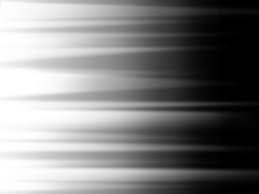
\includegraphics[width=0.3\textwidth]{images/fuzzy.jpeg}

\includegraphics[width=0.3\textwidth]{images/circ2.png}
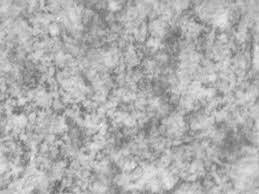
\includegraphics[width=0.3\textwidth]{images/cloud.jpeg}
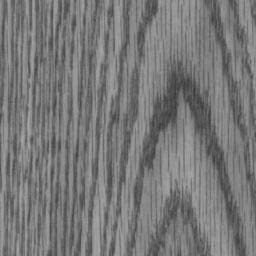
\includegraphics[width=0.3\textwidth]{images/wood.jpg}
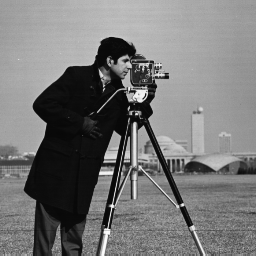
\includegraphics[width=0.3\textwidth]{images/cameraman.png}
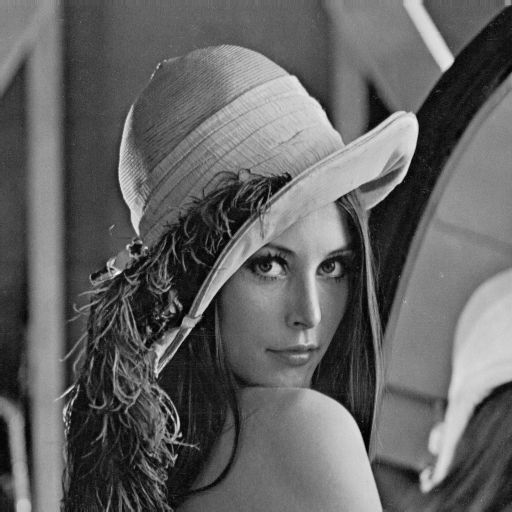
\includegraphics[width=0.3\textwidth]{images/lena.jpg}
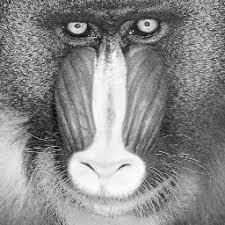
\includegraphics[width=0.3\textwidth]{images/baboon.jpeg}
\caption{\label{fig:imgs}The images used to test the approximating capability of the different networks.}
\end{figure}

\subsubsection{Synthetic images}

\paragraph{}As expected, a reasonably large network easily learns simple synthetic images. On Figure~\ref{fig:circ2}, its performance can be seen.

\begin{figure}[h]
\centering

\includegraphics[width=0.3\textwidth]{images/circ2.png}
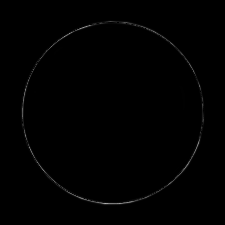
\includegraphics[width=0.3\textwidth]{images_old/circ2e.png}

\includegraphics[width=0.3\textwidth]{images_old/circ2o.png}
\caption{\label{fig:circ2}Synthetic image result. The left image is the original, the middle one is the squared error and the right one is the output of the network.}
\end{figure}

\subsubsection{Texture images}

\paragraph{}This is a more interesting case. Because of its repetitive behavior, it contains less information than a general real-world image. Yet, because of its inner structure, the network fails to grasp this repetition and still tries to approximate areas independently. 

\paragraph{}On Figure~\ref{fig:wood} we can see an acceptable performance. On the right side of the image, the network was able to recognize the wooden pattern, but on its left side, where high frequencies are dominating, it can not do anything.

\begin{figure}[h]
\centering
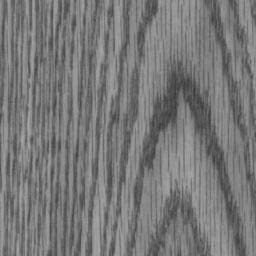
\includegraphics[width=0.3\textwidth]{images/wood.jpg}
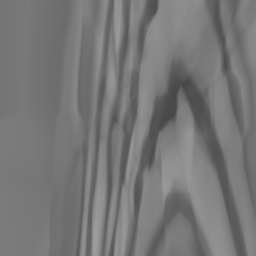
\includegraphics[width=0.3\textwidth]{images_old/woodo.png}
\caption{\label{fig:wood}On this result, we can clearly see how miserably the network is failing to approximate the high frequency parts of the image.}
\end{figure}

\paragraph{}On Figure~\ref{fig:steel}, we can see a bad performance. The networks' only real achievement is the approximation of the lighting: the background of the image is darker in the upper right corner and lighter in the lower left. We can see that it tried to do something with the "real information", but again, could not grasp its pattern, only some parts of it. 

\begin{figure}[h]
\centering
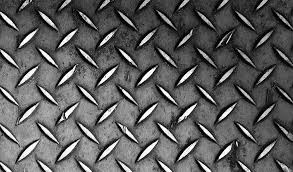
\includegraphics[width=0.3\textwidth]{images_old/steel.jpeg}
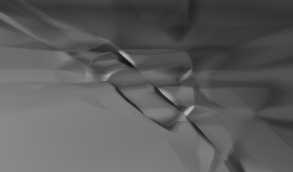
\includegraphics[width=0.3\textwidth]{images_old/steelo.png}
\caption{\label{fig:steel}On this result, we can clearly see how miserably the network is failing to approximate the high frequency parts of the image.}
\end{figure}

\paragraph{}On Figure~\ref{fig:pebbles} we cannot see anything. The network could not find any areas which are worth caring about. The image is quite random indeed, but there are patterns in it. For the network, the biggest problem was probably the too small surfaces of the similar color regions.

\begin{figure}[h]
\centering
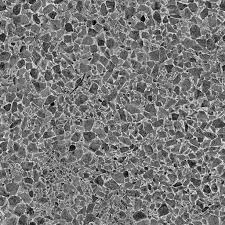
\includegraphics[width=0.3\textwidth]{images_old/pebbles.jpeg}

\includegraphics[width=0.3\textwidth]{images_old/pebbleso.png}
\caption{\label{fig:pebbles}On this result we can clearly see how miserably the network is failing to approximate the high frequency parts of the image.}
\end{figure}

\subsubsection{Real world images}

\paragraph{}The real question is: how well does it perform for natural images? And the answer is: it depends on the image. As we saw earlier, the network can only draw lines. If there are large similar colored regions, it gives much better results.

\section{Conclusion}
Pyramid that contains a typical yet cool conclusion (yeah, we did this and that and it's working, time to celebrate!), draw actual conclusions from our results (i.e. are deeper networks experimentally truly better than shallow ones as our intuition suggested? how and why?) and suggests improvements that could be made over what we already did. Future work should also be mentioned.

\bibliographystyle{plain}
\bibliography{bibTRP}

\end{document}